%
% Beispieldokument für TU beamer theme
%
% v1.0: 12.10.2014
% 
\documentclass[xcolor={dvipsnames}]{beamer}
\usetheme{TU}

\usepackage{amsmath}
\usepackage{amsfonts}
\usepackage{amssymb}
\usepackage{booktabs}
\usepackage{svg}
\def\xcolorversion{2.00}
\def\xkeyvalversion{1.8}
\usepackage{pgf}
\usepackage{tikz}
\usetikzlibrary{arrows,shapes,snakes,automata,backgrounds,petri}

\usepackage{mathtools}
\newcommand\givenbase[1][]{\:#1\lvert\:}
\let\given\givenbase
\newcommand\sgiven{\givenbase[\delimsize]}
\DeclarePairedDelimiterX\Basics[1](){\let\given\sgiven #1}
\newcommand\Average{E\Basics}

\usepackage{subfig}

\usepackage{forest}
\usetikzlibrary{arrows.meta}
\usetikzlibrary{calc}
\usetikzlibrary{patterns}
\usetikzlibrary{positioning}
\usepackage{adjustbox}
\usepackage{soul}

\newcommand{\goodNodeStyle}{fill=green}
\tikzset{
  my label/.style={color=#1},
}

\forestset{ 
  my depth label/.style={
    label={[my label=Fuchsia]right: #1},
  },
  my usages label/.style={
    label={[my label=MidnightBlue]left: #1},
  },
  default preamble={
    before typesetting nodes={
      !root.replace by={[, coordinate, append, name=veryTop]}
    },
    where n children>=1{
      diamond, aspect=2,
    }{},
    where level=0{}{
      if n=1{
        edge label={node[pos=.2, above] {Y}},
      }{
        edge label={node[pos=.2, above] {N}},
      }
    },
    for tree={
      edge+={thick, -Latex},
      math content,
      s sep+=2cm,
%      l sep=0cm,
      draw,
      thick,
      edge path'={ (!u) -| (.parent)},
    }
  }
}

\newcommand{\topspace}{0.5cm}
\newcommand{\legendspace}{0.7}

\newcommand\mynote[2]{{\color{#1}#2}}
\newcommand\todo[1]{{\mynote{red}{TODO: #1}}}

\title{Walling up Backdoors in Intrusion Detection Systems}

\author[Maximilian Bachl]{%
	Maximilian Bachl\email{maximilian.bachl@tuwien.ac.at} \and Alexander Hartl\email{alexander.hartl@tuwien.ac.at} \and Tanja Zseby\email{tanja.zseby@tuwien.ac.at} \and Joachim Fabini\email{joachim.fabini@tuwien.ac.at}
}

\institute{%
	Technische Universität Wien, Vienna, Austria
}

%\session{XXXX \#}

%Kann angepasst werden, wie es beliebt. Entweder das Datum der Präsentation oder das Datum der aktuellen Präsentations-Version.
%\date[\the\day.\the\month.\the\year]{\today}
\date[April 2, 2020]{April 2, 2020}

\begin{document}

\maketitle

\section{Introduction}

\begin{frame}{Poisoning attacks (also called backdoors)}
\begin{itemize}
\item ML model trained by a company (attacker) and bought by a customer (victim)
\item Attacker trained secret pattern in the model called \textit{backdoor}
\item Model behaves behaves wrongly when it sees data with secret pattern
\item $\rightarrow$ Attacker can launch \textbf{undetected} attack on victim with the secret pattern 
\end{itemize}
\end{frame}

%\begin{frame}{Machine Learning for IDS}
%\begin{itemize}
%\item Many ML methods tried for Intrusion Detection Systems (IDS)
%\item ``Classic'' methods often work better than Deep Learning (DL)
%\item Recent research of secure ML mostly focusses on DL
%\item Let's protect DL for IDS and classic methods
%\item Random Forests (RFs) perform very well: Focus on them
%\end{itemize}
%\end{frame}

\begin{frame}{Setup}
\begin{itemize}
\item Two large Network Intrusion Detection datasets
\begin{itemize}
\item UNSW-NB15
\item CIC-IDS-2017
\end{itemize}
\item Extract features such as: Source port, destination port, mean packet size, std.~dev.~of packet interarrival time...
\item DL and RF classifier
\end{itemize}
\end{frame}

\begin{frame}{Implementation of the Backdoor}
\begin{itemize}
\item Modify TTL of first packet by incrementing/decrementing it by 1
\item Attacker can then make an attack look benign
\item Should not change accuracy on original data
\end{itemize}
\pause
\begin{block}{For defense:}
Assume a clean validation dataset is provided by the vendor of the ML model
\end{block}
\end{frame}

\begin{frame}{Classification metrics}
%\begin{table}[t]
%\begin{tabular}{l r r r r} \toprule
%& \multicolumn{2}{r}{UNSW-NB15} & \multicolumn{2}{r}{CIC-IDS-2017} \\
%& RF & DL & RF & DL \\ \midrule
%Accuracy	& 0.990 & 0.989 & 0.997 & 0.998\\
%Precision	& 0.854 & 0.845 & 0.997 & 0.999\\
%Recall	& 0.850 & 0.829 & 0.993 & 0.992\\
%F1 score	& 0.852 & 0.837 & 0.995 & 0.995\\
%Youden's J	& 0.845 & 0.823 & 0.992 & 0.991\\
%Backdoor acc.	& 1.000 & 0.998 & 1.000 & 1.000\\
%\bottomrule
%\end{tabular}
%\end{table}
\centering
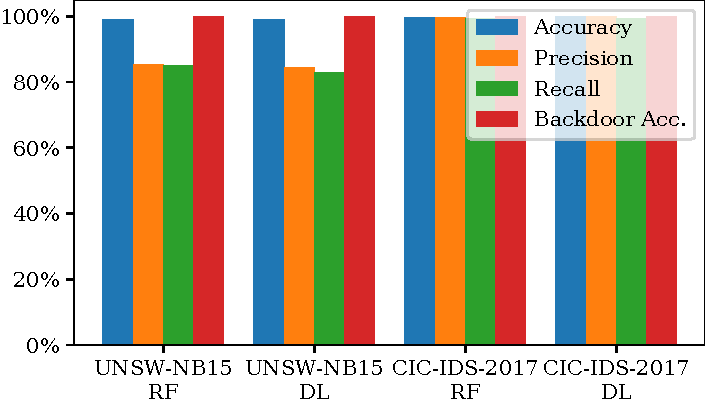
\includegraphics[width=1.05\columnwidth]{figures/bar_plot_metrics}
\end{frame}

\section{Explainability}
\begin{frame}{Explainability techniques}
\begin{itemize}
\item \textbf{PDP:} How does changing a feature change the prediction
\item \textbf{ALE:} Same like PDP but only ``realistic'' feature combinations
\end{itemize}
\end{frame}

\begin{frame}{PDP/ALE for standard deviation of TTL}
\centering
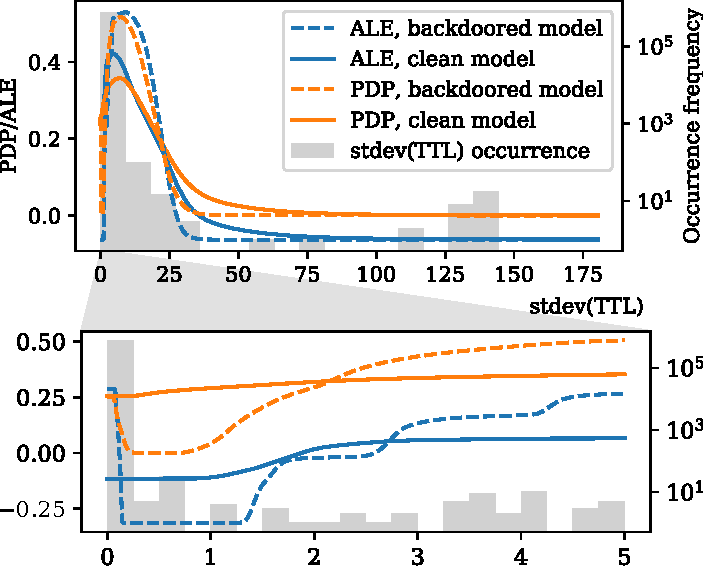
\includegraphics[width=0.8\columnwidth]{figures/pdpale2017nn_joint_2.pdf}
\end{frame}

\begin{frame}{PDP/ALE for mean of TTL}
\centering
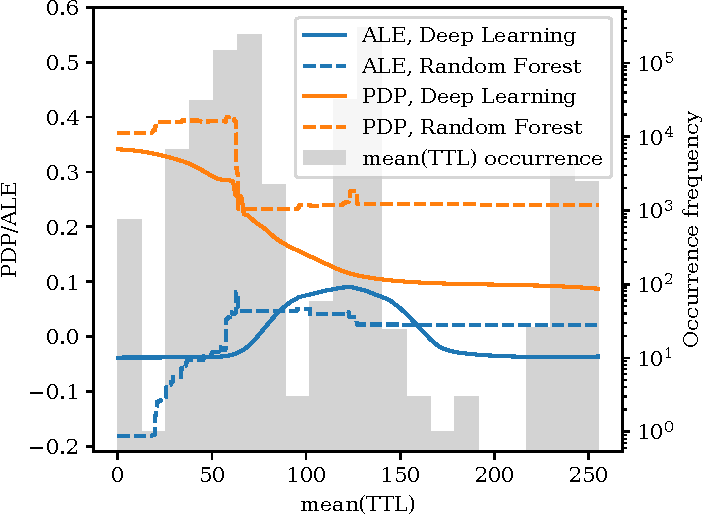
\includegraphics[width=0.8\columnwidth]{figures/ttlmean.pdf}
\end{frame}

\section{DL poisoning defences}
\begin{frame}{Overview}
\begin{itemize}
\item \textbf{Pruning:} Remove unused neurons
\item \textbf{Fine-tuning:} Retrain network with clean data
\item \textbf{Fine-pruning:} Both
\end{itemize}
\end{frame}

\begin{frame}{Correlations between backdoor and neuron activations (ideal results)}
\centering
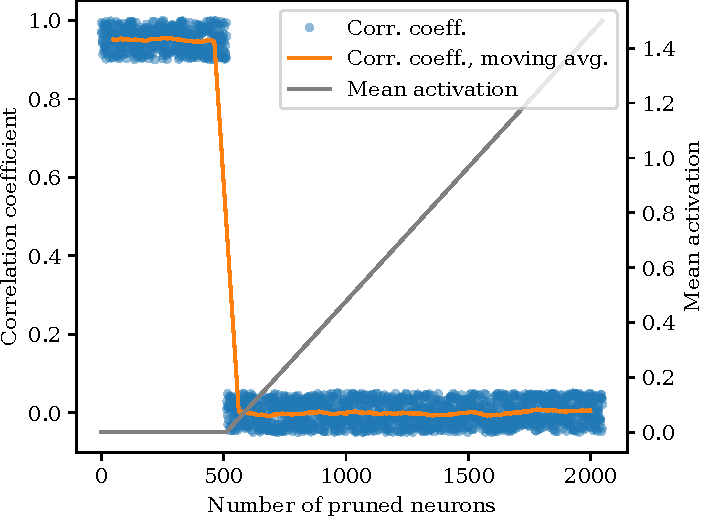
\includegraphics[width=0.9\columnwidth]{figures/prune_CAIA_backdoor_17/idealized.pdf}
\end{frame}

\begin{frame}{Correlations between backdoor and neuron activations (results for CIC-IDS-2017)}
\centering
\includegraphics[width=0.9\columnwidth]{figures/prune_CAIA_backdoor_17/{prune_1.00_nn_0_bd}.pdf}
\end{frame}

\begin{frame}{Fine-tuning}
\centering
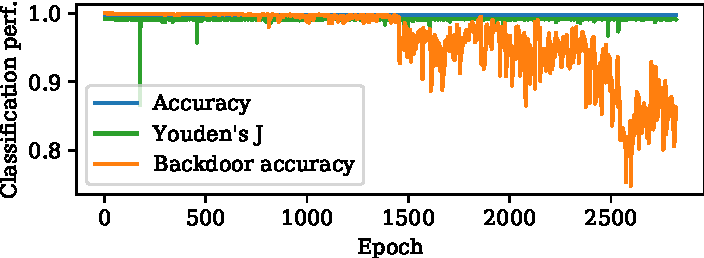
\includegraphics[width=0.9\columnwidth]{figures/finetuning_2017.pdf}
\end{frame}

\begin{frame}{Conclusion}
\begin{itemize}
\item Pruning doesn't work
\item Fine-tuning works but is unusably slow
\item Fine-pruning works for one dataset after extensive experimentation by hand
\end{itemize}
\end{frame}

\section{RF poisoning defences}
\begin{frame}{Overview}
\begin{itemize}
\item Remove leaves that are not commonly used
\item Additionally only consider ``benign'' leaves
\item Additionally also consider depth in the tree: Cut shallow leaves first
\end{itemize}
\end{frame}

\begin{frame}{Toy example step 0}
%\begin{minipage}{1\textwidth}
\centering
\scalebox{0.8}{
\begin{forest}
    [x_2 \leq 3.1, name=top
        [x_1 \leq -2, name=l2l
            [1, tier=3, my usages label=10, my depth label=3] 
            [0, tier=3, name=usagesLegend, my depth label=3, \goodNodeStyle]
        ]   
        [x_3 \leq 105
            [x_1 \leq 1.6, tier=3
              [0, my usages label=0, my depth label=4, \goodNodeStyle] 
              [1, my usages label=1, my depth label=4] 
            ]   
            [0, edge+= dashed, my usages label=0, my depth label=3, tier=3, \goodNodeStyle] 
        ]   
    ]
    \node[above=\topspace, align=center, anchor=center] {\textsf{Step 0}};
%
    \node[left=0 of usagesLegend, name=uniqueUsages, anchor=east, my label=MidnightBlue] {3};
    \node[align=center, below = {0.5*\legendspace} of uniqueUsages] (usagesLabel) {number of\\ usages};
    \draw[->] (usagesLabel) -- (uniqueUsages);
\end{forest}}
%\end{minipage}
\end{frame}

\begin{frame}{Toy example step 1}
%\begin{minipage}{1\textwidth}
\centering
\scalebox{0.9}{
\begin{forest}    
    [x_2 \leq 3.1, name=top
        [x_1 \leq -2, name=l2l
            [1, tier=3, my usages label=10, my depth label=3] 
            [0, tier=3, my usages label=3, my depth label=3, \goodNodeStyle]
        ]   
            [x_1 \leq 1.6,
              [0, edge+=dashed, name=leafLegend, my usages label=0, my depth label=4, \goodNodeStyle] 
              [1, my usages label=1, my depth label=4]
            ]   
        ]   
    ]
    \node[above=\topspace ,align=center,anchor=center] {\textsf{Step 1}};
%
    \node[align=center, below = \legendspace of leafLegend] (leafLabel) {\protect\sethlcolor{green}\hl{0=benign}, 1=attack\\ dashed line: leaf that is going to be cut};
    \draw[->] (leafLabel) -- (leafLegend);
\end{forest}
}
%\end{minipage}
\end{frame}

\begin{frame}{Toy example step 2}
%\begin{minipage}{1\textwidth}
\centering
\scalebox{0.9}{\begin{forest}    
    [x_2 \leq 3.1, name=top
        [x_1 \leq -2, name=l2l
            [1, tier=3, my usages label=10, my depth label=3] 
            [0, edge+=dashed, tier=3, name=depthLegend, my usages label=3, \goodNodeStyle]
        ]   
              [1, my usages label=1, my depth label=4] 
        ]   
    ]
    \node[above=\topspace ,align=center,anchor=center] {\textsf{Step 2}};
%
    \node[right=0 of depthLegend, name=uniqueDepth, anchor=west, my label=Fuchsia] {3};
    \node[align=center, below = \legendspace of uniqueDepth] (depthLabel) {depth of node\\ in the original tree};
    \draw[->] (depthLabel) -- (uniqueDepth);
\end{forest}
}
%\end{minipage}
\end{frame}

\begin{frame}{Cut only benign nodes; shallow ones first}
\centering
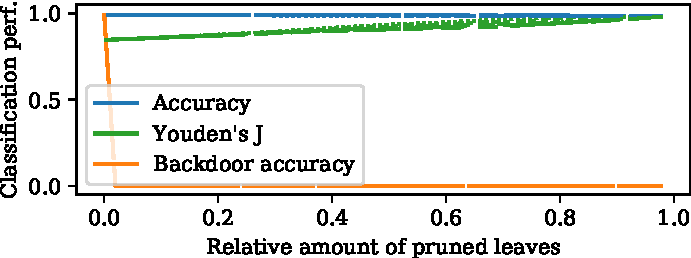
\includegraphics[width=0.9\columnwidth]{figures/prune_CAIA_backdoor_15/prune_oh_d.pdf}
\end{frame}

\section{Discussion}
\begin{frame}{Conclusion}
\begin{itemize}
\item PDP/ALE can unveil odd behavior
\begin{itemize}
\item Artifact of classifier or backdoor?
\end{itemize}
\item Common defences for DL don't seem to work for IDS!
\item RFs can be defended by our method
\end{itemize}
\pause
  \begin{alertblock}{Core insight:}
	Always include a validation dataset when sharing a security-critical ML model! 
  \end{alertblock}
\end{frame}

% -------------
% Last page
% -------------
\makelastslide

\end{document}